
\documentclass{article}[11pt]

\usepackage[utf8]{inputenc}
\usepackage[margin=1in]{geometry}
 \usepackage{setspace} \onehalfspacing
\setlength\parindent{0pt}
\setlength{\parskip}{1em}
\setcounter{secnumdepth}{0}
\usepackage{outlines}
\usepackage{graphicx}
\usepackage{caption}
\captionsetup{justification=centering, width=5in}
\graphicspath{ {imgs} }
\usepackage[normalem]{ulem}
\usepackage{hyperref}
\usepackage{color,soul}

\usepackage{comment}
\pagenumbering{gobble}

\usepackage[
backend=biber,
style=apa,
citestyle=authoryear,
sorting=nyt,
]{biblatex}
\addbibresource{photo_essay.bib}

\title{Ninoofsepoort, an opportunity lost to capital?}
\author{Carla Hyenne}
\date{}

\begin{document}

\newgeometry{margin=0.5in, top=1in}

\maketitle

\begin{figure}[h!]
	\centering
	\captionsetup{labelformat=empty}
	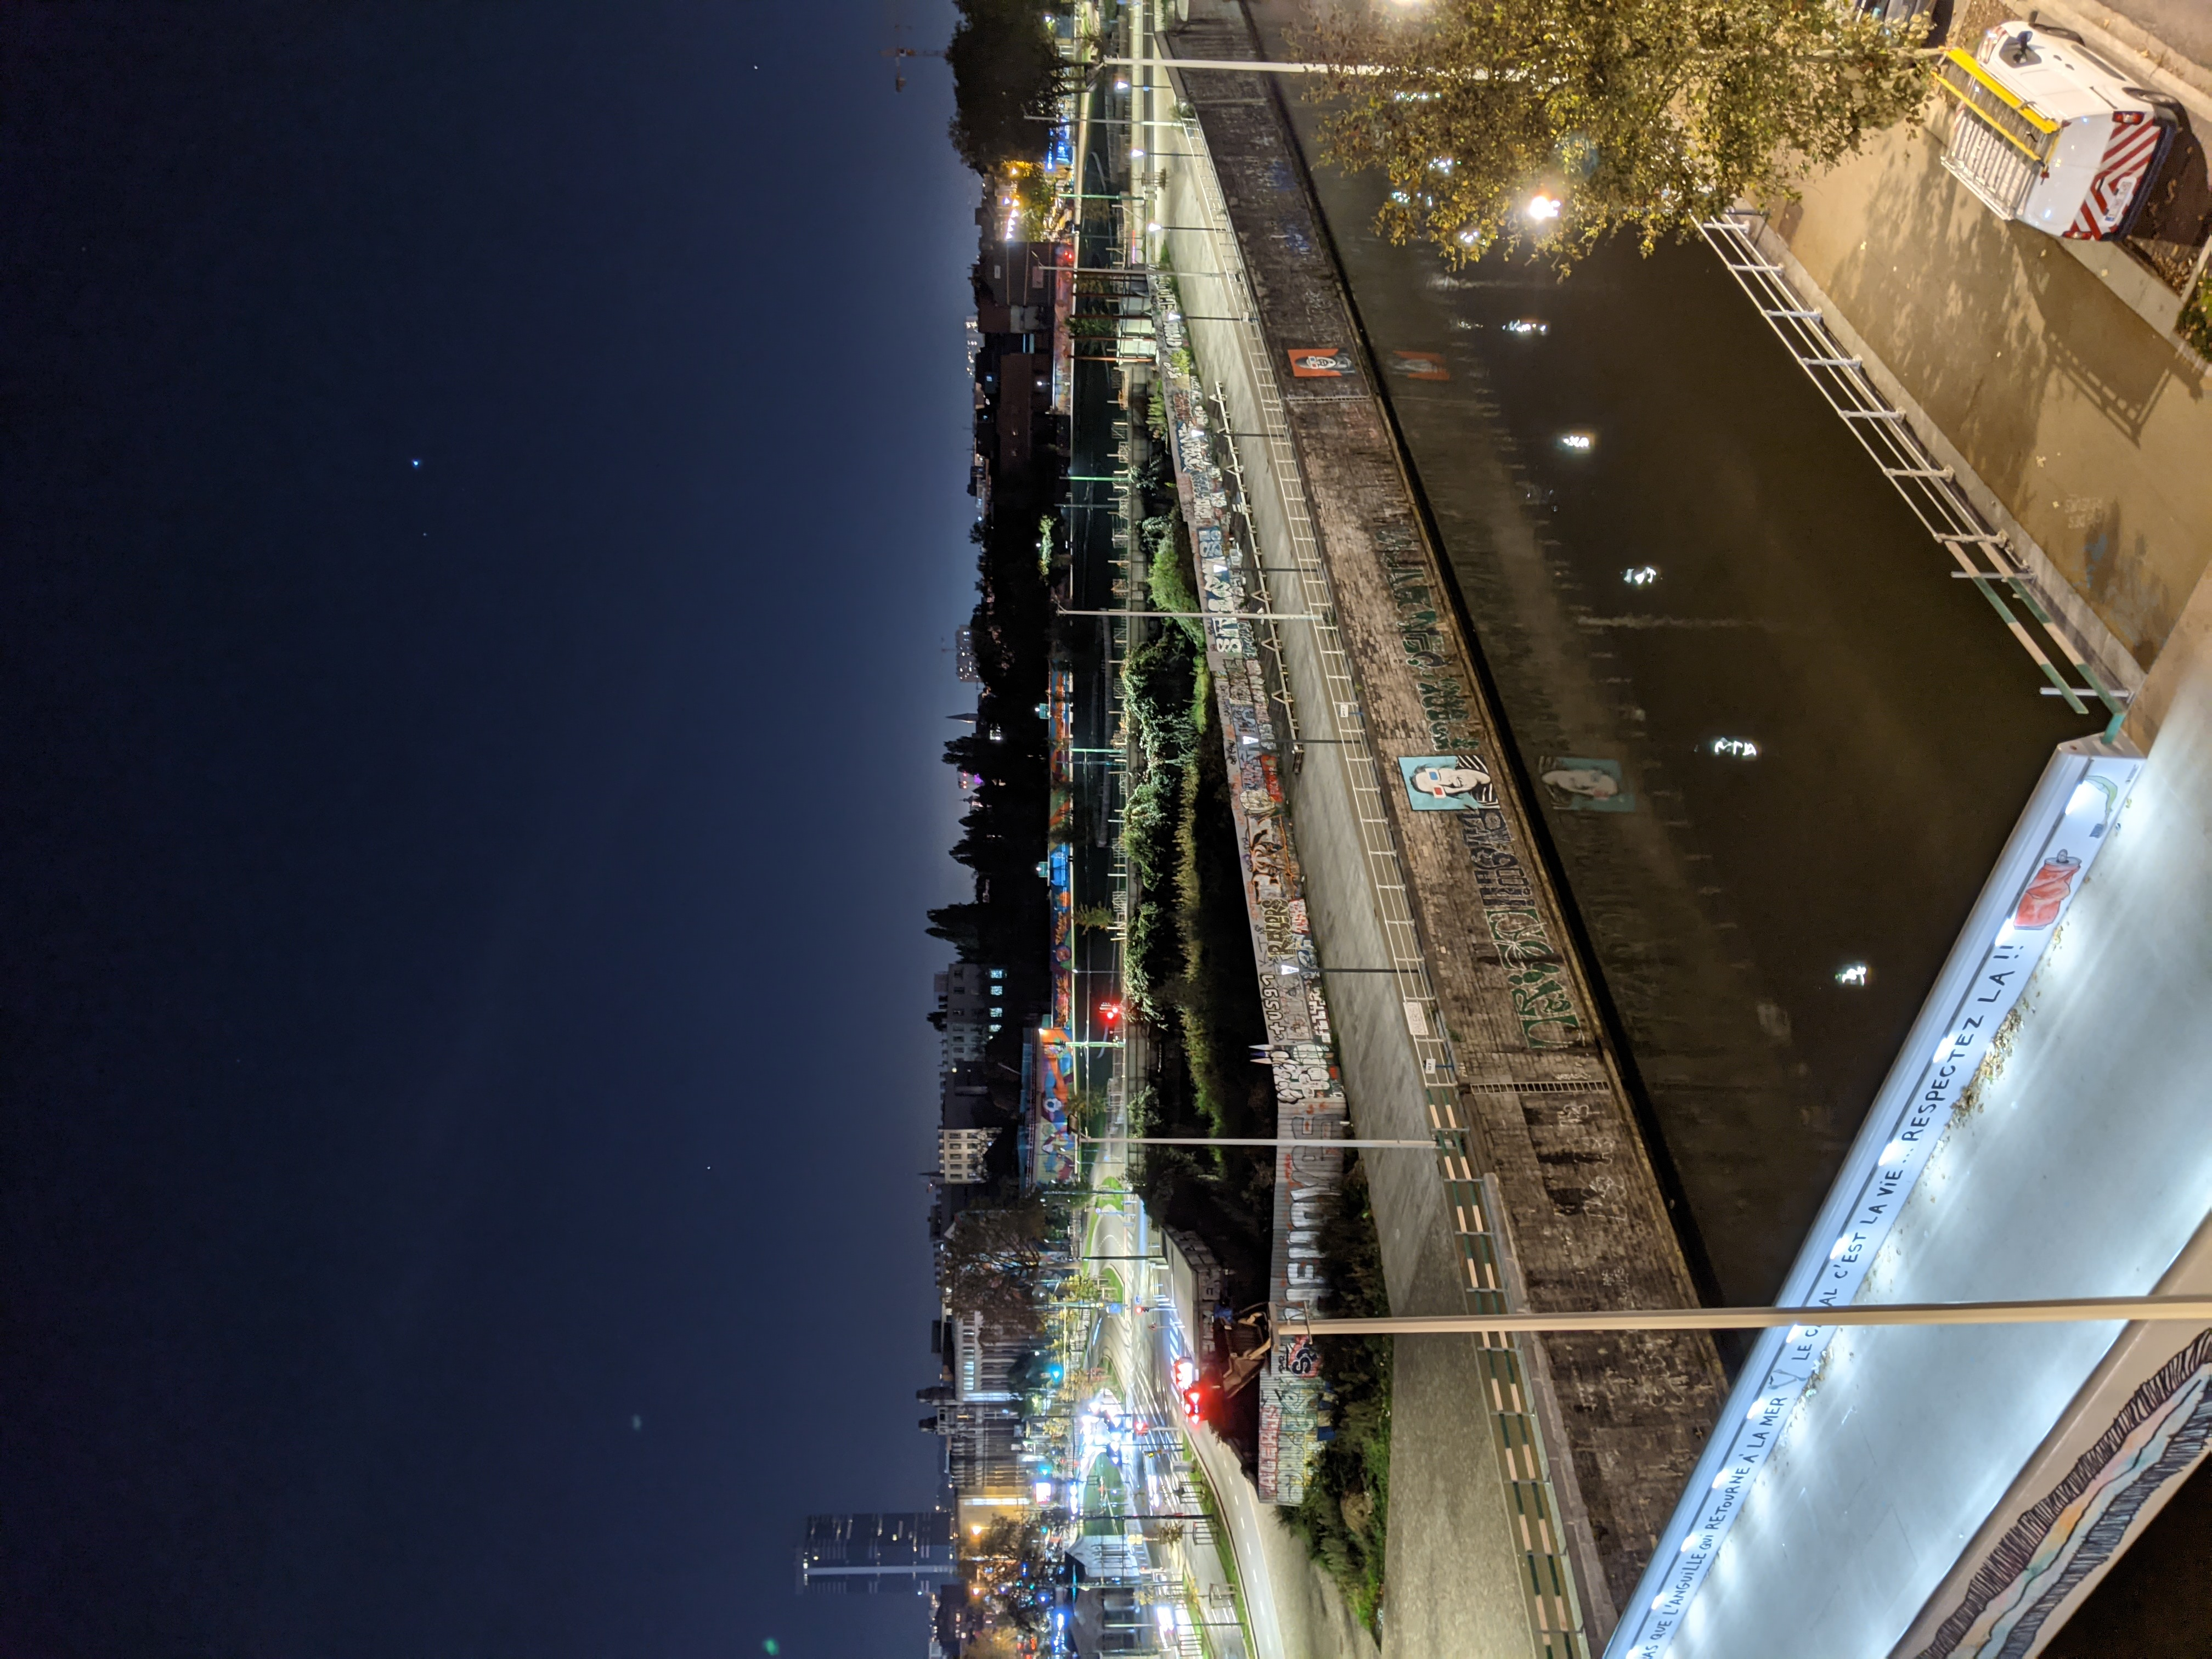
\includegraphics[width=0.85\textwidth, angle=-90]{bxl_canal_far}
	\caption{A view over Ninoofsepoort, taken at night from the terrace of the MIMA museum. From the foreground to the background, we see: the canal over the Petite Senne; an art project from Antoine Caramalli along the canal walls; an undeveloped, overgrown, fenced off plot of land; to its left, tram lines which delimit the Sint-Jans-Molenbeek commune from Brussels Capital commune; further behind, the Ninoofsepoort Park; and the very brightly lit Rue Heyvaert.}
\end{figure}

\restoregeometry

\pagebreak

\begin{comment} 

History of the ninoofsport: 
- what it used to be, why it is now empty, when and who decided to build something on top
- interesting that this triangle of land is ambiguous on land use maps and zoning maps

What can become of ninoofsepoort:
- what does the land use map permit?
- where is the ninoofsepoort located, and what would make sense in this space? comment on the street art, that reminds everyone of the location of ninoofsepoort in molenbeek
- who are the stakeholders? the city, the residents (who are diverse), private investors
- how is it inscribed in the canal redevelopment plan? definitely part of the canal, as it is located right on it; the park will be 
- talk about gentrification of the area: was the MIMA there before (where the photo is taken from), is the park just a plan for attracting private developers?
- what are the aspirations of ninoofsepoort, and how do these integrate into the canal plan? ambiguous goals

What is planned for the left over triangle of land:
- what is the surface area of it, 
- a park was already developed: but for who? minimal infrastructure and furniture, although very well used by molenbeek residents
- was the park part of the plan to attract investors to the plot of land in question?

Relation to course
- investment/disinvestment?
- part of the canal project, and the long park project, which is a gentrification of molenbeek? 

Other notes:
- Citizen Participation? Consultations citoyennes - citizen participation\marginpar{Lecture 5}

- From Urban Analysis
	- PAD: strategic plan, but also gives them the power to change the law in their own advantage; a way for the power that be to do what they want, and circumvent the laws that they usually have to respect; but also a tool for the developers to do what is efficient

- Relate to lecture 5, and gentrification: using MIMA as a regeneration project

- Keywords? Creative and capitalist destruction

- Original wording: ``véritable lieu de convivialité et d’attractivité pour toutes les populations''

% The project, inscribed in the broader canal redevelopment scheme, is a state-led initiative to rebrand the area and make it attractive for a new population with better means.

\end{comment} 

The photo is a view over Ninoofsepoort, or Ninoof's Door. The name of this triangular plot of land is symbolic. Located on the edge of the Brussels' canal, it was once a city gate that provided entry to the historical city centre of Brussels. Unused since the late 20th century, Ninoofsepoort today is at the same time a break in Brussels' urban fabric, and a fantastic opportunity for development. It represents an area of roughly 25.000 $m^2$, only ten minutes walking distance from the Grand Place, in a dense city with limited space, and in a neighbourhood targeted as a zone for urban renovation \parencite{perspective2020zru}. As such, Ninoofsepoort is high stakes for the city.

The photo itself was taken from the MIMA, a museum of contemporary art opened in 2016. One of the museum's aims was to give the neighbourhood of Molenbeek a new image. An image of culture and dynamism, intended to overrule the prevailing sentiment of insecurity and fear. The faces with 3D glasses visible on the canal walls are a satirical piece by artist Antoine Caramalli, entitled `The Big Molenbeek Show'. The faces of Molenbeek are staring back in irony at those looking onto the neighbourhood, following the ``giant media circus''\parencite{antoine2016canal} after the 2016 Paris attacks carried out by terrorists from Molenbeek.

I think Caramalli, an inhabitant of Molenbeek himself, perfectly summarises the neighbourhood as the ``home of the poor, the artists, the immigrants and the tourists, fertile ground of mixity and culture''\parencite{antoine2016canal}.
This poetic description conveys Ninoofsepoort's multi-faceted politicoeconomic, sociocultural position with many actors, including inhabitants, politicians, planners, and private investors.

Visible in the back of the photo is the Ninoofsepoort park, which was constructed in 2018. Though minimally furnished, the park is well used by a diversity of inhabitants and provides relief from a lack of green space in an otherwise highly dense neighbourhood.
Adjacent to the park, visible by overgrown shrubs and surrounded by a graffiti-covered fence, sits an undeveloped private plot of land which is the centre of much debate. 
This raises the question: was the park planned for the inhabitants, or to attract private investors in a location with unrealised potential?

In 2016, the government mandated perspective.brussels (hereinafter referred to as Perspective), an NGO, to evaluate the land and plan its development \parencite{diagnosticNinove}. Perspective formulated a goal for Ninoofsepoort - to make it ``a real place of conviviality and attractiveness for all populations'' \parencite{perspectiveNinove}. Three aspects stand out: conviviality, attractiveness, and all populations. 
The land was then sold to the private real estate developer Besix RED, and a PAD (Guiding Development Plan) was put in place.

The PAD is a tool that has the power to overrule regulations, and is being used to facilitate the real estate development. The land use has been changed to allow private housing and to build at a height of 90 meters. The reasons presented for the PAD are to anchor Ninoofsepoort within Brussels' small ring, already dotted with high-rise buildings; to give Ninoofsepoort an identity; and to improve the quality of the urban space.

\textbf{Conviviality, Attractiveness, All populations?}

Given Molenbeek's socio-economic situation, it is not hard to be critical of the Ninoofsepoort PAD. Besix RED has planned three housing towers that will comprise of 270 private housing units, along with 240 parking spots. However, none of the units will be social housing, and the mere plan for so much parking implies who will move in - a population who needs a car on a regular basis to get to work - and confirms the ambitions of the real estate developer to attract a different class.

The plans emphasise the importance of creating open, public space on the ground floor of the towers, with metropolitan equipment such as socio-cultural infrastructure and daycares. But, for whom is this space, and this equipment? In light of the fact that the current population is poor and working class, it will be a challenge to create public space within the private complex that truly accommodates diverse uses and populations. Perversely and contrary to intentions, this promotion for diversity, and the development of Ninoofsepoort park, encourage gentrification by attracting real estate developers like Besix RED and middle to upper classes able to buy the new housing units.

The location's extremely attractive potential makes it vulnerable to speculators. For the city, it is attractive to sell or lease the land, and reap the benefits of taxation and income from wealthier residents. But these would not really be \textit{benefits}. Trickle down effects have long been disproven \parencite{required}, and current inhabitants would likely be gone before they see any benefit.

Furthermore, this development is a stark contrast to the resident's demands for their neighbourhood when they were consulted in 2014 $\rightarrow$ todo:expand.

Molenbeek is one of the poorest neighbourhoods of Brussels, one of the densest in Europe, and in desperate need of green and public spaces, and public equipment \parencite{ieb2019ninove}. Considering the need for public investment, and that the privately developed towers won't have social housing, it is clear that the plan did not aim to include the population of Molenbeek, who could not afford the units. 
The argument of social mix, modernisation, and a supra-local vision prevailed.

Investing money in a disadvantaged neighbourhood tends to accelerate gentrification and displacement if there are no policies to reduce unemployment, and improve living conditions for existing residents \parencite{required}.
Moreover, Ninoofsepoort is being used as a strategic site to integrate a multitude of projects that are part of the Canal Plan. These plans, like the PAD Heyvaert, will further displace residents and especially local businesses important to the area, like the car dealerships in Rue Heyvaert.
With Besix RED's towers, the vicious cycle of investment, gentrification, and displacement will perpetuate.

%The housing development would contribute to the gentrification of Molenbeek, by raising the attractiveness of the area, thus rising prices, and displacing people and businesses who either cannot afford the new rent or are forced out for the sake of urban regeneration.

\textbf{Hope for the Right to the City}

Given the above, it is clear that there is no intention to address the concerns of those who currently live in the area, but rather, to cater to the aspirations of wealthier classes. 
This photo encapsulates the failure of the city to meet the challenges of Molenbeek, but what it does not show is the impressive citizen mobilisation against property speculation on Ninoofsepoort that took place. The private developer plans to sell the land, and the authorities may exclude it the PAD, thus lowering the risk for speculation \parencite{ieb2020ninove}.

Ninoofsepoort is an opportunity for the Brussels' government to show more ambition in the social housing developments, given the enormous demand and embarrassingly low supply. So far, it has fallen victim to ``Bruxellisation'', where the interests of private investors are prioritised over those of local inhabitants, justified by the necessity to modernise. But it need not be this way.

\pagebreak

\printbibliography 

\end{document}
